We used the open-source software package Gephi~\cite{gephi2009} to compute centralities on the citation network, and Mathematica to run linear regressions.

\subsubsection{Total citation count}
\label{sectionCitcount}
The total of in-degrees in the citation network of a scholar's papers is a simple measure of his degree of recognition and influence. We regressed 2010 base salary against total citation count up to 2009 and years since Ph.D. (secondary regressor). From table~\ref{tableTotalCitCount}, we conclude that both regressors' coefficients differ significantly from 0, and particularly salary is significantly related to total citation count, at the 1\% level.

\begin{table}[h]
	\centering
	\label{tableTotalCitCount}
	\caption{Results of linear regression with total citation count}
	\begin{tabular} {|l|c|c|}\hline
		$R^2 \approx 0.606$  & \text{estimate} &  \text{$p$-value} \\ \hline
		\text{constant} & $57078.5$ & $1.63\cdot10^{-9}$\\ \hline
		\text{years since Ph.D.} & $2431.5$ & $2.02\cdot10^{-10}$ \\ \hline
		\text{total citations} & $5.062$ & $9.61\cdot10^{-3}$\\ \hline
	\end{tabular}
\end{table}

\begin{figure}[h]
	\label{figTotalcit}
	\centering
	%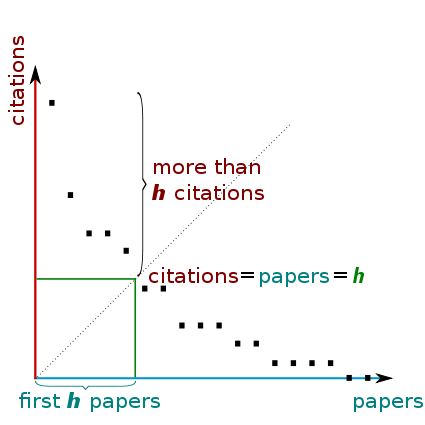
\epsfig{file=figures/hindex.eps}
	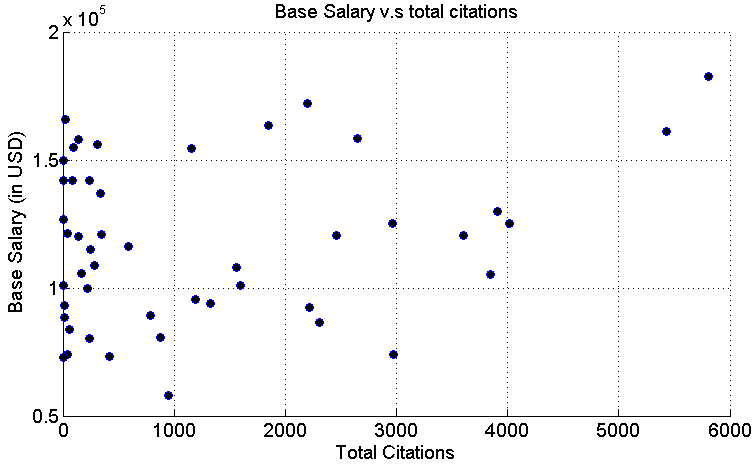
\includegraphics[width=0.5\textwidth]{figures/totalcit.png}
	\caption{Plot of base salary versus citations per year.}
\end{figure}

\subsubsection{Citations per year}
\label{sectionCitperyear}
@@@@@@@@@@@
Whereas citation counts accumulate over time, it might instead matter more the @@@@@@@@@@@
@@@@@@@@@ What exactly is being regressed on? Citations per year of what?///////////
% Citation counts accumulate over time. To illustrate: imagine a professor published a paper 20 years ago that got immediate attention with many citations, but had little long-term impact. The paper would indeed be of value, but @@@@what?
We therefore regress salary on citations per year (as well as years since Ph.D.) \figref{figCitperyear}. From the results in Table~\ref{tableCitperyear}, we reject the null hypothesis to find a correlation between salary and citations per year significant at the 2\% level.

\begin{table}[h]
	\centering
	\label{tableCitperyear}
	\caption{Results of linear regression with citations per year.}
	\begin{tabular} {|l|c|c|}\hline
		$R^2 \approx 0.601$  & \text{estimate} &  \text{$p$-value} \\ \hline
		\text{constant} & $56349.2$ & $1.21\cdot10^{-8}$\\ \hline
		\text{years since Ph.D.} & $2447.57$ & $7.12\cdot10^{-10}$ \\ \hline
		\text{Citations Per Year} & $45.8953$ & $1.65\cdot10^{-2}$\\ \hline
	\end{tabular}
\end{table}

\begin{figure}[h]
	\label{figCitperyear}
	\centering
	%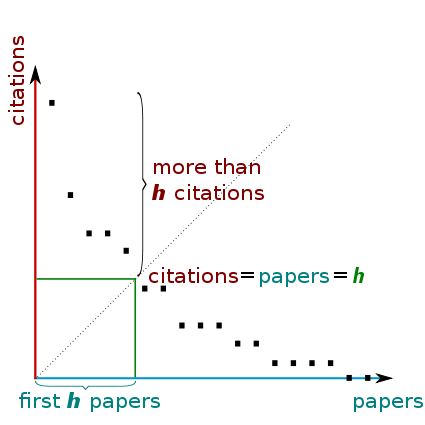
\epsfig{file=figures/hindex.eps}
	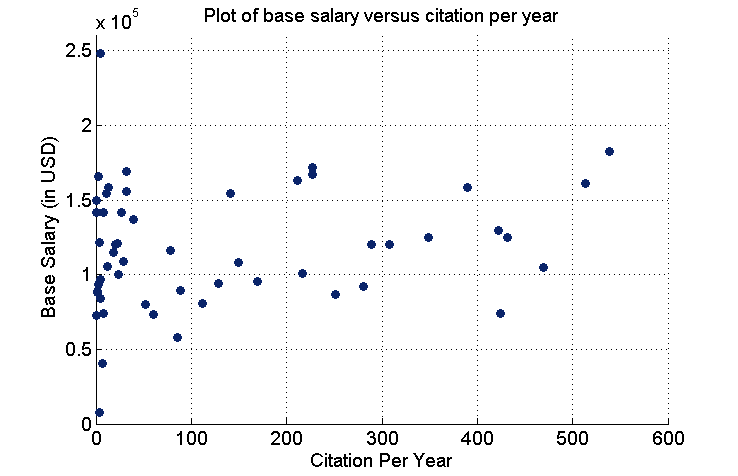
\includegraphics[width=0.5\textwidth]{figures/citperyr.png}
	\caption{Plot of base salary versus citations per year}
\end{figure}



\subsubsection{PageRank}
\label{sectionPageRank}
PageRank~\cite{page1999} is an eigenvector centrality measure. It tries to capture the relative importance of a node based on the rank of its neighbors.

\begin{equation}
	\label{eqnPageRank}
	PageRank(A) = \frac{1-\alpha}{N} + \alpha \sum_{i\in\mathcal{N}_A}\frac{PageRank(i)}{d_{out}(i)}
\end{equation}
where, $\alpha$ is the damping factor, $N$ is the total number of nodes, $\mathcal{N}_A = \{i : i\ \text{is a neighbor of A} \}$, $d_{out}$ is the out-degree of node $i$. From the equation~\ref{eqnPageRank} we see that PageRank weighs each in-coming edge by the fraction of the rank of the source node.

In our study, we use $\alpha = 0.85$ which is the typical value of damping factor used in most PageRank computations. Also we set our error tolerance limit to $10^{-5}$ to compute the PageRank numerically using iGraph~\cite{iGraph2006}. We added the PageRank of individual papers to obtain productivity of professor and regressed it against base salary. Table~\ref{tablePageRank} gives the output of this regression, and we see that the p-value is too high to reject null hypothesis.

\begin{table}[h]
	\centering
	\label{tablePageRank}
	\caption{Results of linear regression with PageRank}
	\begin{tabular} {|l|c|c|}\hline
		$R^2 \approx 0.562$  & \text{estimate} &  \text{$p$-value} \\ \hline
		\text{constant} & $61447.5$ & $1.39\cdot10^{-9}$\\ \hline
		\text{years since Ph.D.} & $2420.96$ & $3.03\cdot10^{-9}$ \\ \hline
		\text{PageRank} & $1.1362\cdot10^{6}$ & $0.1945$\\ \hline
	\end{tabular}
\end{table}


\subsubsection{Change in citation count}
\label{sectionDeltacit}

The results in section~\ref{sectionCitcount} and~\ref{sectionCitperyear} suggest a correlation between citations and base salary. Salary of a professor is not stagnant. There will be revisions every few years. It would be interesting to see how change in citation count is correlated to change in base salary. From the UC system, we see that there is a change in base salary every two years, in even year. So, we computed biyearly change from $2004$ to $2010$ in salary and citation count and ran a linear regression. Since we are concerned with change in the quantities, we follow the following model,
\begin{equation}
	salary = \beta_1 \Delta\text{Citation}.
\end{equation}

From table~\ref{tableDeltacit}, we see that the p-vale is very low and hence we can reject the null hypothesis.  

\begin{table}[h]
	\centering
	\label{tableDeltacit}
	\caption{Results of linear regression with biyearly change in citation and salary}
	\begin{tabular} {|l|c|c|}\hline
		$R^2 \approx 0.270$  & \text{estimate} &  \text{$p$-value} \\ \hline
		\text{$\Delta Citation$} & $33.4899$ & $6.14\cdot10^{-12}$ \\ \hline
	\end{tabular}
\end{table}

\begin{figure}[h]
\label{figDeltacit}
\centering
%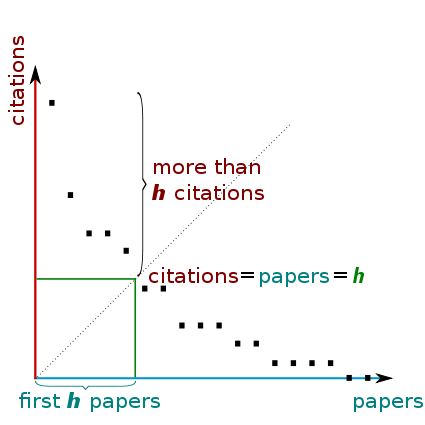
\epsfig{file=figures/hindex.eps}
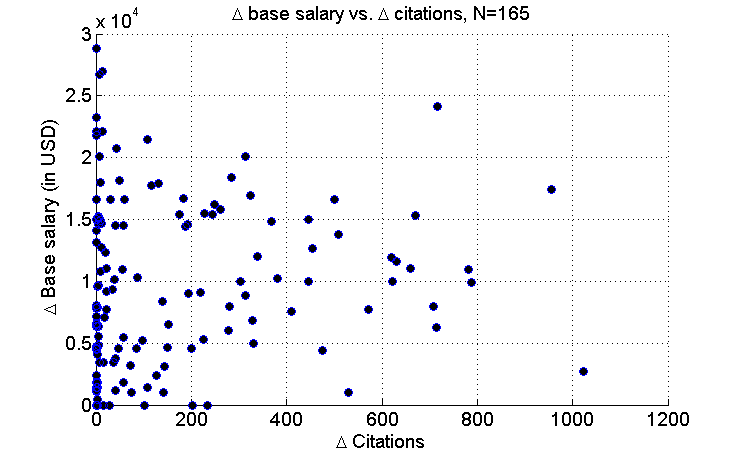
\includegraphics[width=0.5\textwidth]{figures/deltacitations.png}
\caption{Plot of biyearly change in base salary versus change in citations.}
\end{figure}

\subsubsection{$h$-index (of citation count)}

The $h$-index was introduced by Hirsh~\cite{hirsh2005Hindex} as a measure of the impact of a researcher's works:
\begin{definition}
	\label{defHindex}
	A scholar's $h$-index is the largest integer $h$ such that each of his top $h$ papers have centrality at least $h$. For a centrality measure $c$, we denote the $h$-index as $h(c)$.
\end{definition}

\begin{figure}[h]
\label{figHindex}
	\centering
	%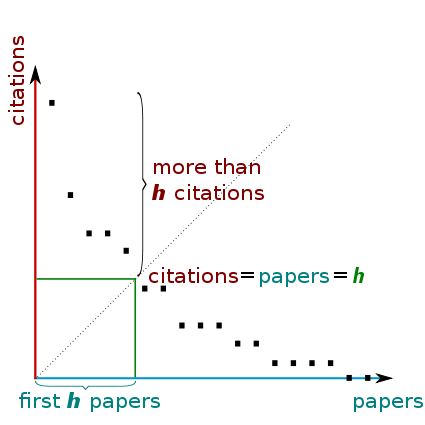
\epsfig{file=figures/hindex.eps}
	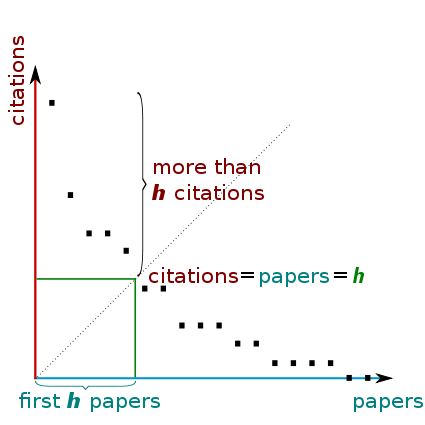
\includegraphics[width=0.4\textwidth]{figures/hindex.png}
	\caption{Computing the $h$-index (\small{Courtesy: Wikipedia})}.
\end{figure}

We computed $h(citations)$ for the professors based on the total citation count of each of their papers. We regressed base salary against $h(citations)$ (using years since Ph.D. as a secondary variable), with results in Table~\ref{tableHindex}. The regression result does not support any correlation between salary and $h(citations)$ at the 5\% level.

\begin{table}[h]
	\centering
	\label{tableHindex}
	\caption{Results of linear regression with $h$-index}
	\begin{tabular} {|l|c|c|}\hline
		$R^2 \approx 0.550$  & \text{estimate} &  \text{$p$-value} \\ \hline
		\text{constant} & $54787.5$ & $6.07\cdot10^{-7}$\\ \hline
		\text{years since Ph.D.} & $2593.7$ & $1.7\cdot10^{-9}$ \\ \hline
		\text{$h(citations)$} & $262.509$ & $0.39$\\ \hline
	\end{tabular}
\end{table}


\subsubsection{$g$-index (of citation count)}

In 2006, Leo Egghe~\cite{egghe2006Gindex} suggested a refinement of the $h$-index. We define
\begin{definition}
	\label{defGindex}
	The $g$-index is the largest integer $g$ such that the top $g$ articles (ordered by centrality) have a total centrality of at least $g^2$.
\end{definition}

That is,
\begin{equation}
	\label{eqnGindex}
	g^2 \leq \sum_{i\leq g} c_i
	\iff
	g \leq \frac{1}{g} \sum_{i\leq g} c_i
\end{equation}
where $c_i$ is the centrality of paper $i$. Equivalently, an author's top $g$ papers have on average at least $g$ citations each.

\begin{figure}[h]
	\label{figGindex}
	\centering
	%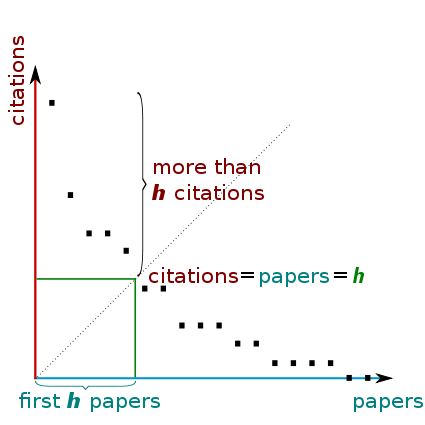
\epsfig{file=figures/hindex.eps}
	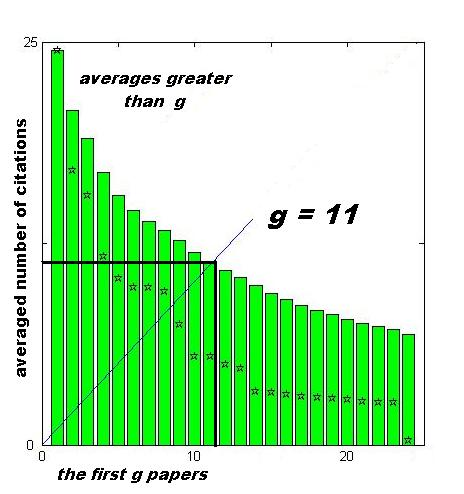
\includegraphics[width=0.4\textwidth]{figures/Gindex1.png}
	\caption{Computing the $g$-index (\small{Courtesy: Wikipedia})}.
\end{figure}

We computed $g(citations)$ for the professors based on the total citation count of each of their papers. We regressed base salary against $g(citations)$ (using years since Ph.D. as a secondary variable), with results in Table~\ref{tableGindex}. The regression result does not support any correlation between salary and $g(citations)$ at the 5\% level.

\begin{table}[h]
	\centering
	\label{tableGindex}
	\caption{Results of linear regression with $g$-index}
	\begin{tabular} {|l|c|c|}\hline
		$R^2 \approx 0.547$  & \text{estimate} &  \text{$p$-value} \\ \hline
		\text{constant} & $55951.3$ & $1.32\cdot10^{-7}$\\ \hline
		\text{years since Ph.D.} & $2602.33$ & $5.83\cdot10^{-10}$ \\ \hline
		\text{$g$(citations)} & $90.8829$ & $0.55$\\ \hline
	\end{tabular}
\end{table}

